\documentclass[conference,a4paper]{IEEEtran}
\IEEEoverridecommandlockouts
\usepackage[utf8]{inputenc}
\usepackage[T1]{fontenc}
\usepackage[spanish,es-noshorthands,es-tabla]{babel}
\usepackage{amsmath,amssymb}
\usepackage{graphicx}
\usepackage{booktabs}
\usepackage{multirow}
\usepackage{xcolor}
\usepackage{tikz}
\usetikzlibrary{arrows.meta,positioning,fit}
\usepackage[hidelinks]{hyperref}
\usepackage{cite}
\decimalpoint
\newcommand{\pmsd}[2]{#1\,$\pm$\,#2}

\begin{document}

\title{CNN frente a Vision Transformer con pocos datos:\\
detección de enfermedades en hojas de papa fotografiadas en campo}

\author{\IEEEauthorblockN{[Nombre completo 1], [Nombre completo 2], [Nombre completo 3], [Nombre completo 4]}
\IEEEauthorblockA{Maestría en Inteligencia Artificial, Unidad de Posgrado FIIS\\
Universidad Nacional de Ingeniería, Lima, Perú\\
MIA-203 Redes Neuronales y Aprendizaje Profundo --- Equipo [N]}}

\maketitle

\begin{abstract}
Diagnosticar a tiempo las enfermedades de la papa es clave para un cultivo central en la seguridad alimentaria del Perú. Los modelos de visión suelen entrenarse con fotos de laboratorio, pero en campo hay fondos variados, manos, sombras y plásticos. Estudiamos si, con solo 2\,112 imágenes de entrenamiento tomadas en campo y 7 clases desbalanceadas, conviene una red convolucional (ResNet-50) o un Vision Transformer (ViT-S/16), y cuánto aporta el preentrenamiento en ImageNet. Primero auditamos el conjunto de datos público: encontramos 55 pares de duplicados exactos (6 de ellos con etiquetas contradictorias) y casi-duplicados, y construimos una partición 70/15/15 por grupos sin fuga de datos. Comparamos 6 configuraciones con 3 semillas cada una, frente a un Random Forest con descriptores de color y textura y una CNN pequeña. Preentrenados, ResNet-50 y ViT-S/16 alcanzan macro-F1 de \pmsd{0.843}{0.012} y \pmsd{0.853}{0.013} en prueba, sin diferencia significativa según la prueba de McNemar ($p\geq0.16$). Ambos superan ampliamente al Random Forest (\pmsd{0.464}{0.021}). Sin preentrenamiento, el ViT cae a \pmsd{0.499}{0.028}, por debajo de la ResNet-50 entrenada desde cero (\pmsd{0.642}{0.007}). Es decir, con pocos datos el preentrenamiento importa más que la arquitectura. Grad-CAM muestra que la ResNet concentra su atención en la lesión, mientras que la CNN pequeña a veces usa atajos del fondo. Publicamos el código, la partición, los pesos y una demo reproducible.
\end{abstract}

\begin{IEEEkeywords}
Vision Transformer, ResNet, transferencia de aprendizaje, enfermedades de la papa, Grad-CAM, pocos datos.
\end{IEEEkeywords}

%=====================================================================
\section{Introducción}
La papa es uno de los cultivos más importantes del Perú y del mundo. Las enfermedades foliares, como la rancha (\textit{Phytophthora infestans}), las virosis o el daño por insectos, reducen el rendimiento si no se detectan a tiempo. El diagnóstico visual depende de especialistas que no siempre están disponibles en campo. Por eso, un clasificador de imágenes ejecutable desde un celular podría servir como apoyo temprano.

El aprendizaje profundo ya logra exactitudes casi perfectas en conjuntos de laboratorio como PlantVillage~\cite{mohanty2016plant,ferentinos2018plant}, con hojas aisladas sobre fondo uniforme. Sin embargo, esos modelos se degradan con fotos de campo~\cite{mohanty2016plant}. El conjunto de Shabrina \textit{et al.}~\cite{shabrina2024potato} reúne 3\,076 fotos de hojas de papa tomadas en campo en Java Central (Indonesia), en 7 clases. Sus líneas base reportan exactitudes de solo 0.68--0.74.

Al mismo tiempo, los Vision Transformers (ViT)~\cite{dosovitskiy2021vit} han desplazado a las CNN en muchos problemas. Sin embargo, se sabe que necesitan muchos datos o un preentrenamiento fuerte~\cite{dosovitskiy2021vit,touvron2021deit,steiner2022howtotrain}. Esto plantea una pregunta práctica para equipos con pocos datos y poco cómputo: \emph{¿qué arquitectura elegir y cuánto depende el resultado del preentrenamiento?}

\textbf{Contribuciones.}
\begin{enumerate}
\item \textbf{Auditoría y partición sin fuga.} Auditamos el conjunto de datos público: 110 imágenes en 55 pares de duplicados exactos, 12 de ellas con etiquetas contradictorias, y 64 imágenes en grupos de casi-duplicados. Construimos una partición 70/15/15 por grupos, reproducible con un comando.
\item \textbf{Comparación controlada.} Comparamos ResNet-50 y ViT-S/16 (preentrenados y desde cero), una CNN pequeña y un Random Forest, con 3 semillas, métricas adecuadas al desbalance (macro-F1) y prueba de significancia (McNemar).
\item \textbf{Ablación del preentrenamiento.} Cuantificamos que aporta $+0.355$ de macro-F1 al ViT y $+0.201$ a la ResNet.
\item \textbf{Interpretabilidad y demo.} Analizamos los errores con Grad-CAM, incluyendo una medida de concentración de los mapas, y publicamos un demo reproducible en Colab con el modelo final.
\end{enumerate}

%=====================================================================
\section{Trabajos relacionados}
\textbf{CNN y transferencia de aprendizaje.} Las redes residuales~\cite{he2016resnet} permitieron entrenar CNN profundas mediante conexiones de identidad. Su preentrenamiento en ImageNet~\cite{deng2009imagenet} es el punto de partida estándar con pocos datos. En plantas, Mohanty \textit{et al.}~\cite{mohanty2016plant} y Ferentinos~\cite{ferentinos2018plant} alcanzaron más de 99\,\% de exactitud en PlantVillage, pero advierten que el desempeño cae con imágenes de campo. Nuestro trabajo usa precisamente fotos de campo.

\textbf{Transformers en visión.} El Transformer~\cite{vaswani2017attention} reemplaza la convolución por autoatención. El ViT~\cite{dosovitskiy2021vit} lo aplica a parches de $16\times16$ píxeles y supera a las CNN solo cuando se preentrena en conjuntos muy grandes. DeiT~\cite{touvron2021deit} y Steiner \textit{et al.}~\cite{steiner2022howtotrain} mostraron que la regularización y el preentrenamiento compensan en parte la falta de sesgo inductivo. Raghu \textit{et al.}~\cite{raghu2021vitsee} encontraron que el ViT integra información global desde las primeras capas, a diferencia de la CNN. Nosotros medimos este contraste en un problema real con solo $\sim$2\,100 imágenes.

\textbf{Papa en condiciones no controladas.} Shabrina \textit{et al.}~\cite{shabrina2024potato} publicaron el conjunto que usamos y reportaron líneas base con una sola partición 90/10: ResNet-50 obtiene 0.682 de exactitud y EfficientNetV2-B3, 0.736. Sangar y Rajasekar~\cite{sangar2025potato} combinan EfficientNet-LITE con un SVM en entornos diversos. Ninguno de los dos trabajos controla duplicados entre particiones, reporta varias semillas ni compara con Transformers.

\textbf{Interpretabilidad y atajos.} Grad-CAM~\cite{selvaraju2017gradcam} localiza las regiones que más influyen en una clase. Su aplicación a ViT es menos fiel que en CNN~\cite{chefer2021transformer}, lo que consideramos al interpretar. Geirhos \textit{et al.}~\cite{geirhos2020shortcut} describen el \emph{aprendizaje por atajos}: decidir por pistas espurias del fondo. Lo observamos en nuestra CNN pequeña.

%=====================================================================
\section{Metodología}
\begin{figure*}[t]
\centering
\resizebox{\textwidth}{!}{%
\begin{tikzpicture}[node distance=4mm, font=\footnotesize,
  caja/.style={draw, rounded corners=2pt, align=center, minimum height=10mm, inner sep=3pt, fill=#1},
  caja/.default=white, flecha/.style={-{Latex[length=2mm]}, thick}]
\node[caja=gray!10] (raw) {3\,076 fotos\\1500$\times$1500\\7 clases};
\node[caja=gray!10, right=of raw] (dedup) {Deduplicación\\sha256 (exactos)\\dHash $\leq4$ (casi)};
\node[caja=gray!10, right=of dedup] (split) {Partición por grupos\\70/15/15, semilla 42\\2112 / 450 / 453};
\node[caja=gray!10, right=of split] (aug) {256$\to$224 px\\aumento: recorte,\\volteo, rotación, color};
\node[caja=blue!8, right=10mm of aug, yshift=9mm] (cnn) {ResNet-50 / CNN pequeña\\(convolución local)};
\node[caja=orange!12, right=10mm of aug, yshift=-9mm] (vit) {ViT-S/16: 196 parches\\+ autoatención global};
\node[caja=green!8, right=10mm of cnn, yshift=-9mm] (eval) {Mejor época por\\macro-F1 de validación\\$\Rightarrow$ prueba (1 vez)};
\node[caja=gray!10, right=of eval] (xai) {Grad-CAM,\\McNemar,\\demo};
\draw[flecha] (raw) -- (dedup); \draw[flecha] (dedup) -- (split); \draw[flecha] (split) -- (aug);
\draw[flecha] (aug.east) -- (cnn.west); \draw[flecha] (aug.east) -- (vit.west);
\draw[flecha] (cnn.east) -- (eval.west); \draw[flecha] (vit.east) -- (eval.west); \draw[flecha] (eval) -- (xai);
\end{tikzpicture}}
\caption{Flujo del estudio. La partición se hace por grupos de casi-duplicados para evitar fuga de datos; el conjunto de prueba solo se usa una vez, al final de cada corrida.}
\label{fig:pipeline}
\end{figure*}

\subsection{Datos}
Usamos el \textit{Potato Leaf Disease Dataset in Uncontrolled Environment}~\cite{shabrina2024potato,shabrina2023mendeley} (Mendeley Data, licencia CC BY 4.0). Contiene 3\,076 fotos JPG de $1500\times1500$ píxeles tomadas en campo. Las 7 clases son bacteria, hongos (\textit{fungi}), sana, nematodos, plaga de insectos (\textit{pest}), \textit{Phytophthora} y virus. El desbalance es marcado: de 67 imágenes (nematodos) a 740 (hongos) tras la limpieza.

\textbf{Auditoría.} Calculamos el hash sha256 de cada archivo y encontramos 110 imágenes que forman 55 pares de duplicados exactos. En 6 pares, la misma foto aparece en dos clases distintas. Eliminamos esas 12 imágenes, por tener etiqueta contradictoria, y 49 copias redundantes, de modo que quedan 3\,015. Además, calculamos un \textit{hash} perceptual dHash de 64 bits sobre la versión de $256\times256$. Unimos con \textit{union-find} los pares con distancia de Hamming $\leq4$, lo que da 64 imágenes en grupos de casi-duplicados.

\textbf{Partición.} Hacemos una partición estratificada por grupo 70/15/15 (semilla 42): 2\,112 imágenes de entrenamiento, 450 de validación y 453 de prueba. Cada grupo de casi-duplicados cae completo en una sola partición, para que el modelo no se evalúe con variantes de fotos que ya vio. La validación se usa para elegir la mejor época y el modelo final; la prueba se evalúa una única vez por corrida.

\subsection{Modelos}
\textbf{Línea base clásica.} Un Random Forest~\cite{breiman2001rf} con 1\,834 descriptores por imagen:
\begin{itemize}
\item Histograma HSV de 48 dimensiones.
\item Medias y desviaciones RGB/HSV (12).
\item HOG~\cite{dalal2005hog} sobre $128\times128$ (1\,764).
\item LBP uniforme~\cite{ojala2002lbp} (10).
\end{itemize}
Usa pesos de clase balanceados y una búsqueda en malla (número de árboles, \texttt{max\_features} y \texttt{min\_samples\_leaf}) elegida por macro-F1 de validación.

\textbf{CNN pequeña} (1.2\,M parámetros), entrenada desde cero. Tiene 4 bloques [Conv$3{\times}3$--BN--ReLU]$\times2$ + MaxPool, con anchos 32--256, seguidos de \textit{pooling} global, \textit{dropout} 0.3 y una capa lineal.

\textbf{ResNet-50}~\cite{he2016resnet} (23.5\,M). Cada bloque aprende un residuo, $\mathbf{y}=\mathcal{F}(\mathbf{x},\{W_i\})+\mathbf{x}$; la convolución impone localidad e invariancia a la traslación.

\textbf{ViT-S/16}~\cite{dosovitskiy2021vit} (21.7\,M). Divide la imagen de $224\times224$ en $N=196$ parches de $16\times16$ y los proyecta a $d=384$ dimensiones. Agrega un token \texttt{[CLS]} y embeddings de posición, y aplica 12 bloques de autoatención multi-cabeza (6 cabezas) con
\begin{equation}
\text{Atención}(Q,K,V)=\mathrm{softmax}\!\left(\frac{QK^\top}{\sqrt{d_h}}\right)V,
\end{equation}
donde cada parche puede atender a todos los demás desde la primera capa.

\textbf{Pesos preentrenados.} Ambos modelos grandes provienen de \texttt{timm}~\cite{wightman2019timm}:
\begin{itemize}
\item ResNet-50: \texttt{resnet50.a1\_in1k}, preentrenada en ImageNet-1k.
\item ViT-S/16: \texttt{vit\_small\_patch16\_224.}\allowbreak\texttt{augreg\_in21k\_ft\_in1k}, preentrenado en ImageNet-21k y ajustado en ImageNet-1k.
\end{itemize}
Reemplazamos la cabeza por una capa de 7 salidas y ajustamos \emph{todos} los parámetros. En la ablación ``desde cero'' usamos la misma arquitectura con inicialización aleatoria.

\subsection{Función de pérdida y entrenamiento}
Para compensar el desbalance usamos entropía cruzada ponderada:
\begin{equation}
\mathcal{L}=-\frac{1}{B}\sum_{i=1}^{B} w_{y_i}\log \frac{e^{z_{i,y_i}}}{\sum_{k=1}^{K}e^{z_{i,k}}},\qquad
w_k=\frac{1/n_k}{\frac{1}{K}\sum_{j}1/n_j},
\end{equation}
donde $n_k$ es el número de imágenes de la clase $k$ en entrenamiento y $K=7$. Así, la clase nematodos (47 imágenes) pesa 3.5 y la clase hongos, 0.32.

\textbf{Optimizador y calendario.} Usamos AdamW~\cite{loshchilov2019adamw} (Tabla~\ref{tab:hp}). La tasa de aprendizaje sube linealmente durante 2 épocas y luego decae con coseno hasta cero:
\begin{equation}
\eta_t=\begin{cases}\eta_{\max}\,\frac{t+1}{T_w}, & t<T_w\\[2pt]
\frac{\eta_{\max}}{2}\Big(1+\cos\frac{\pi(t-T_w)}{T-T_w}\Big), & t\geq T_w\end{cases}
\end{equation}
con $t$ en pasos de minibatch.

\textbf{Configuración común.} Tamaño de lote 32, 40 épocas sin parada temprana, recorte de gradiente a norma 1 y \textit{dropout} 0.2 en la cabeza. La precisión mixta fp16 se usa en ResNet y ViT; la CNN pequeña entrena en fp32 porque en fp16 colapsaba en nuestra GPU local.

\textbf{Aumento de datos.} Recorte aleatorio redimensionado (escala 0.6--1), volteos horizontal y vertical, rotación de $\pm20^\circ$ y variación de brillo, contraste y saturación. Cada configuración se entrena con las semillas 0, 1 y 2.

\begin{table}[t]
\caption{Hiperparámetros (AdamW, lote 32, 40 épocas, 224$\times$224)}
\label{tab:hp}
\centering\small
\begin{tabular}{lccc}
\toprule
Modelo & $\eta_{\max}$ (pre / cero) & \textit{Weight decay} & Parámetros \\
\midrule
CNN pequeña & -- / $10^{-3}$ & 0.01 & 1.2\,M \\
ResNet-50 & $3{\times}10^{-4}$ / $10^{-3}$ & 0.05 & 23.5\,M \\
ViT-S/16 & $10^{-4}$ / $5{\times}10^{-4}$ & 0.05 & 21.7\,M \\
\bottomrule
\end{tabular}
\end{table}

\subsection{Métricas y prueba estadística}
Como las clases están desbalanceadas, la métrica principal es el \textbf{macro-F1}, $\frac{1}{K}\sum_k \mathrm{F1}_k$, que da el mismo peso a cada clase. También reportamos la exactitud balanceada y la exactitud, como media $\pm$ desviación estándar sobre semillas.

Para comparar ResNet-50 y ViT-S/16 con la misma semilla aplicamos la prueba exacta de McNemar~\cite{dietterich1998tests}. Sean $b$ y $c$ las imágenes de prueba que solo acierta uno u otro modelo; bajo $H_0$, $b\sim\mathrm{Binomial}(b+c,\tfrac12)$.

\subsection{Interpretabilidad}
Aplicamos Grad-CAM~\cite{selvaraju2017gradcam}:
\begin{equation}
\alpha_k^c=\frac{1}{Z}\sum_{i,j}\frac{\partial y^c}{\partial A^k_{ij}},\qquad
L^c=\mathrm{ReLU}\Big(\sum_k \alpha_k^c A^k\Big).
\end{equation}
Las capas objetivo son:
\begin{itemize}
\item ResNet-50: el último bloque de \texttt{layer4} (mapa de $7\times7$).
\item CNN pequeña: la última convolución.
\item ViT: la normalización previa al último bloque; descartamos el token \texttt{[CLS]} y reordenamos los 196 tokens en una rejilla de $14\times14$.
\end{itemize}
Para cuantificar la forma de los mapas medimos dos cosas:
\begin{itemize}
\item La \emph{masa top-10\,\%}: fracción de la activación que cae en el 10\,\% de píxeles más activos. Un mapa uniforme da 0.10.
\item La \emph{masa central}: fracción en el cuadrado central, que ocupa el 25\,\% del área. Un mapa uniforme da 0.25.
\end{itemize}

%=====================================================================
\section{Resultados}

\begin{table}[t]
\caption{Resultados en prueba (453 imágenes), media $\pm$ DE sobre 3 semillas. \textbf{Negrita}: mejor.}
\label{tab:main}
\centering\small
\setlength{\tabcolsep}{3pt}
\resizebox{\columnwidth}{!}{%
\begin{tabular}{lccc}
\toprule
Modelo & Macro-F1 & Exact. bal. & Exactitud \\
\midrule
Random Forest (color+HOG+LBP) & \pmsd{0.464}{0.021} & \pmsd{0.452}{0.014} & \pmsd{0.558}{0.010} \\
CNN pequeña (cero) & \pmsd{0.614}{0.011} & \pmsd{0.661}{0.004} & \pmsd{0.630}{0.009} \\
ResNet-50 (cero) & \pmsd{0.642}{0.007} & \pmsd{0.687}{0.013} & \pmsd{0.659}{0.003} \\
ViT-S/16 (cero) & \pmsd{0.499}{0.028} & \pmsd{0.550}{0.019} & \pmsd{0.497}{0.029} \\
ResNet-50 (preentrenada) & \pmsd{0.843}{0.012} & \pmsd{0.845}{0.011} & \pmsd{0.855}{0.005} \\
ViT-S/16 (preentrenado) & \textbf{\pmsd{0.853}{0.013}} & \textbf{\pmsd{0.849}{0.008}} & \textbf{\pmsd{0.869}{0.016}} \\
\midrule
\multicolumn{4}{l}{\textit{Publicado~\cite{shabrina2024potato}: partición 90/10 sin deduplicar, 1 corrida}} \\
ResNet-50 & -- & -- & 0.682 \\
EfficientNetV2-B3 & -- & -- & 0.736 \\
\bottomrule
\end{tabular}}
\end{table}

\subsection{Comparación con las líneas base}
La Tabla~\ref{tab:main} resume las 18 corridas propias (6 configuraciones $\times$ 3 semillas).
\begin{itemize}
\item \textbf{Frente a la línea base clásica:} los dos modelos preentrenados superan al Random Forest en más de 0.37 de macro-F1, y a la CNN pequeña en más de 0.22.
\item \textbf{Frente a lo publicado:} nuestra ResNet-50 preentrenada obtiene 0.855 de exactitud, contra 0.682 en~\cite{shabrina2024potato}. Hay que leer esta comparación con cautela, porque la partición y el protocolo difieren.
\item \textbf{Variabilidad entre semillas:} es baja ($\leq0.013$ de DE en macro-F1) para los modelos preentrenados.
\end{itemize}

\subsection{CNN frente a ViT}
Con preentrenamiento, el ViT-S/16 supera a la ResNet-50 por solo 0.010 de macro-F1, una diferencia menor que la desviación entre semillas. La prueba de McNemar por semilla (Tabla~\ref{tab:mcnemar}) no rechaza $H_0$ en ningún caso ($p=0.38$, 1.00 y 0.16).

Por clase (Fig.~\ref{fig:f1}), los dos modelos se reparten las victorias: el ViT es mejor en \textit{Phytophthora} (0.87 frente a 0.80) y hongos (0.85 frente a 0.82); la ResNet, en virus (0.88 frente a 0.86) y nematodos (0.80 frente a 0.77). Concluimos que, preentrenadas, \textbf{ambas arquitecturas son estadísticamente equivalentes} en este problema.

\begin{table}[t]
\caption{McNemar exacto, ResNet-50 vs ViT-S/16 preentrenados (prueba)}
\label{tab:mcnemar}
\centering\small
\begin{tabular}{cccc}
\toprule
Semilla & Solo ResNet acierta ($b$) & Solo ViT acierta ($c$) & $p$ \\
\midrule
0 & 20 & 27 & 0.38 \\
1 & 24 & 25 & 1.00 \\
2 & 20 & 31 & 0.16 \\
\bottomrule
\end{tabular}
\end{table}

\begin{figure*}[t]
\centering
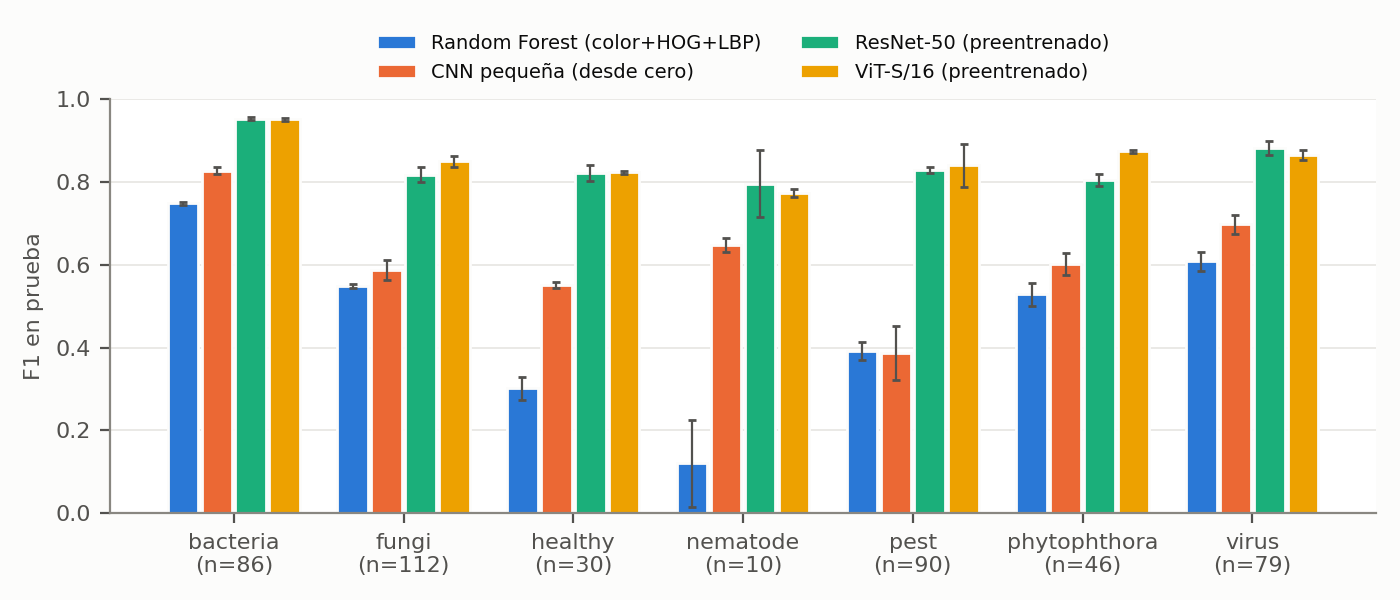
\includegraphics[width=0.82\textwidth]{figs/f1_por_clase.png}
\caption{F1 por clase en prueba (media y DE sobre 3 semillas; $n$ = imágenes de prueba por clase). Los modelos preentrenados dominan en todas las clases; la mayor brecha con las líneas base está en nematodos, sana y plaga.}
\label{fig:f1}
\end{figure*}

\subsection{Ablación: efecto del preentrenamiento}
La Tabla~\ref{tab:abl} aísla el preentrenamiento manteniendo arquitectura, datos, partición e hiperparámetros, y ajustando solo la tasa de aprendizaje.
\begin{itemize}
\item \textbf{Ganancia en el ViT:} $+0.355$ de macro-F1.
\item \textbf{Ganancia en la ResNet:} $+0.201$.
\item \textbf{ViT desde cero:} queda incluso por debajo de la CNN pequeña, que tiene 18 veces menos parámetros, y es el modelo más inestable entre semillas (DE 0.028).
\item \textbf{ResNet desde cero:} supera levemente a la CNN pequeña (0.642 frente a 0.614).
\end{itemize}
Esto coincide con~\cite{dosovitskiy2021vit,touvron2021deit}: sin el sesgo inductivo de localidad, el Transformer necesita aprender desde los datos cómo se relacionan los parches vecinos, y 2\,112 imágenes no alcanzan.

\begin{table}[t]
\caption{Ablación del preentrenamiento (macro-F1 en prueba)}
\label{tab:abl}
\centering\small
\begin{tabular}{lccc}
\toprule
Modelo & Preentrenado & Desde cero & $\Delta$ \\
\midrule
ResNet-50 & \pmsd{0.843}{0.012} & \pmsd{0.642}{0.007} & $+0.201$ \\
ViT-S/16 & \pmsd{0.853}{0.013} & \pmsd{0.499}{0.028} & $+0.355$ \\
\bottomrule
\end{tabular}
\end{table}

\subsection{Análisis de errores}
La Fig.~\ref{fig:conf} muestra la matriz de confusión del ViT preentrenado, sumando las 3 semillas. Los errores se concentran en tres confusiones:
\begin{itemize}
\item \textbf{Plaga $\to$ hongos:} 14\,\% de las fotos de plaga. En ResNet, 11\,\%.
\item \textbf{\textit{Phytophthora} $\to$ hongos:} 12\,\%.
\item \textbf{Nematodos $\to$ hongos:} 17\,\%, con solo 10 imágenes de prueba.
\end{itemize}
Hongos es la clase más numerosa y la de síntomas más variados (manchas necróticas, clorosis), por lo que funciona como ``clase sumidero''. En el Random Forest, el 34\,\% de las fotos de plaga se clasifica como hongos. Además, el 11\,\% de las hojas sanas se confunde con virus, cuyos síntomas tempranos (mosaico leve) son sutiles a $224\times224$.

\begin{figure}[t]
\centering
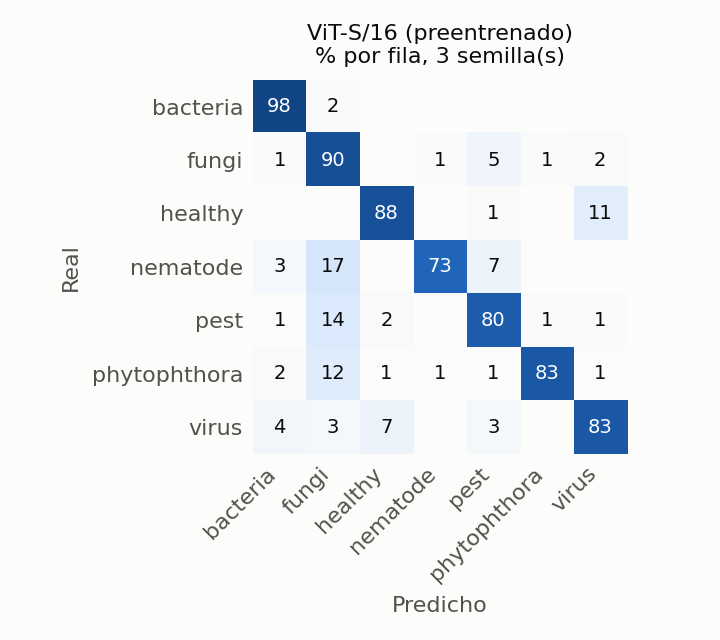
\includegraphics[width=0.86\columnwidth]{figs/confusion_vit_small_pre.png}
\caption{Matriz de confusión del ViT-S/16 preentrenado en prueba (\% por fila, 3 semillas sumadas). Hongos actúa como clase sumidero de plaga, \textit{Phytophthora} y nematodos.}
\label{fig:conf}
\end{figure}

\subsection{Interpretabilidad (Grad-CAM)}
La Fig.~\ref{fig:cam} compara los mapas de los tres modelos sobre las mismas imágenes de prueba; la Tabla~\ref{tab:cam} los cuantifica sobre 22 imágenes.
\begin{itemize}
\item \textbf{ResNet-50:} produce mapas compactos (masa top-10\,\% = 0.50) centrados en la lesión. Por ejemplo, señala la mancha necrótica en \textit{Phytophthora} (fila~3) y la perforación en plaga (fila~4).
\item \textbf{ViT-S/16:} sus mapas son más dispersos (0.29), casi tan repartidos como un mapa uniforme en la región central (0.27 frente a 0.25). Esto es coherente con su atención global~\cite{raghu2021vitsee}, aunque Grad-CAM es menos fiel en Transformers~\cite{chefer2021transformer}. Aun así, en la fila~3 se concentra en la misma lesión que la ResNet.
\item \textbf{CNN pequeña:} muestra \emph{aprendizaje por atajos}~\cite{geirhos2020shortcut}. En la fila~1 acierta ``bacteria'' mirando el plástico de \textit{mulch} del fondo, no la hoja. En la fila~3 predice ``sana'' porque atiende a las nervaduras en lugar de la lesión.
\end{itemize}
Este hallazgo advierte que, en fotos de campo, un acierto no garantiza que el modelo use la evidencia correcta.

\begin{figure}[t]
\centering
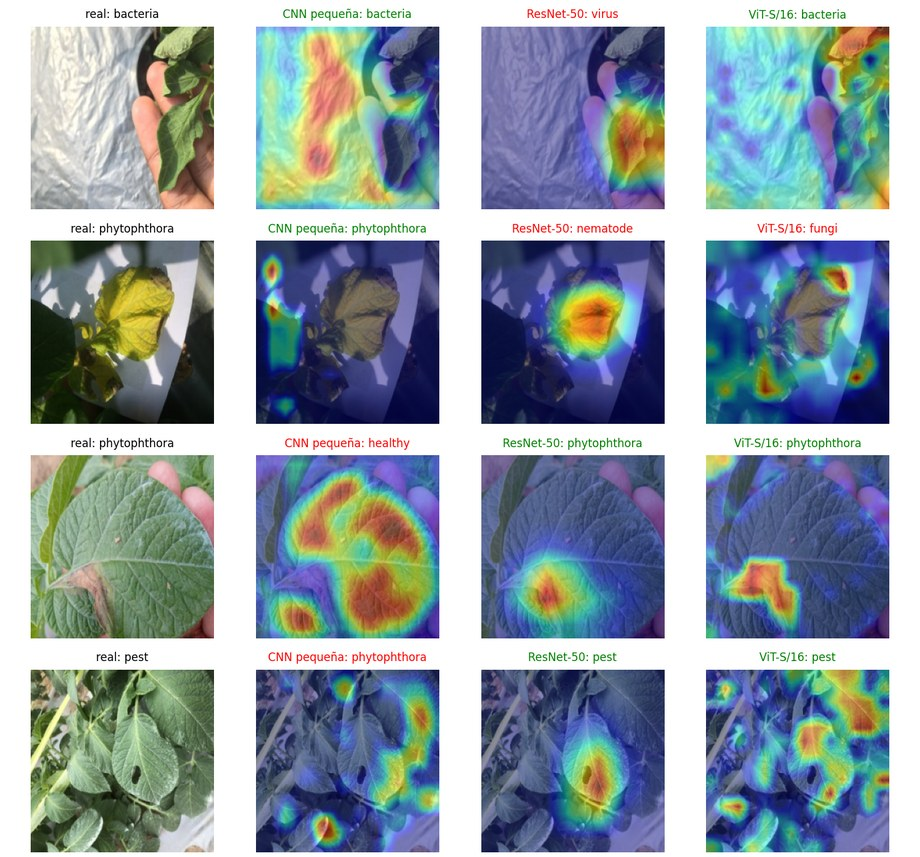
\includegraphics[width=\columnwidth]{figs/gradcam_errores.jpg}
\caption{Grad-CAM en imágenes de prueba (verde = acierto, rojo = error). Fila~1: la CNN pequeña acierta usando el plástico del fondo (atajo). Fila~3: ResNet y ViT localizan la lesión de \textit{Phytophthora}; la CNN pequeña no.}
\label{fig:cam}
\end{figure}

\begin{table}[t]
\caption{Concentración de los mapas Grad-CAM (22 imágenes de prueba)}
\label{tab:cam}
\centering\small
\begin{tabular}{lcc}
\toprule
Modelo & Masa top-10\,\% & Masa central \\
\midrule
CNN pequeña & \pmsd{0.37}{0.18} & \pmsd{0.34}{0.13} \\
ResNet-50 & \pmsd{0.50}{0.11} & \pmsd{0.61}{0.18} \\
ViT-S/16 & \pmsd{0.29}{0.11} & \pmsd{0.27}{0.11} \\
\midrule
Mapa uniforme (referencia) & 0.10 & 0.25 \\
\bottomrule
\end{tabular}
\end{table}

\subsection{Costo computacional}
Usamos dos equipos: Google Colab (Tesla T4, 16\,GB) y una laptop con GeForce GTX 1650 Ti de 4\,GB. Las 21 corridas suman $\approx$5.9\,h de GPU (Tabla~\ref{tab:cost}).
\begin{itemize}
\item \textbf{En la T4:} una corrida de 40 épocas tarda $\approx$15\,min, con un pico de memoria de 1.5\,GB (ViT) y 1.8\,GB (ResNet).
\item \textbf{En la laptop:} la misma corrida de ResNet tarda 66\,min. En esa GPU, la precisión mixta fp16 produjo colapsos (la validación predecía una sola clase), por lo que la CNN pequeña se entrenó en fp32 y las semillas 1 y 2 de la ResNet preentrenada se entrenaron en la T4.
\item \textbf{En inferencia:} el modelo final clasifica una imagen y calcula su Grad-CAM en $\approx$0.2\,s en CPU.
\end{itemize}

\begin{table}[t]
\caption{Costo de entrenamiento (40 épocas por corrida)}
\label{tab:cost}
\centering\small
\setlength{\tabcolsep}{4pt}
\begin{tabular}{llcc}
\toprule
Modelo & Hardware & min/corrida & Corridas \\
\midrule
Random Forest & CPU & 1.8 & 3 \\
CNN pequeña & GTX 1650 Ti & 40.1 & 3 \\
ResNet-50 (pre) & GTX 1650 Ti / T4 & 65.9 / 15.8 & 1 / 2 \\
ResNet-50 (cero) & T4 & 15.9 & 3 \\
ViT-S/16 (pre) & T4 & 14.4 & 3 \\
ViT-S/16 (cero) & T4 & 15.0 & 3 \\
\midrule
\multicolumn{2}{l}{Total GPU} & \multicolumn{2}{c}{$\approx$5.9\,h} \\
\bottomrule
\end{tabular}
\end{table}

\subsection{Modelo final y demo}
Elegimos como modelo final la corrida con mayor macro-F1 de \emph{validación}, sin mirar la prueba: ViT-S/16 preentrenado con semilla 2. Obtuvo 0.929 en validación y, en prueba, 0.864 de macro-F1 y 0.883 de exactitud.

La demo se ejecuta en Colab o en local (Gradio). Recibe una foto, la recorta al centro y devuelve las 3 clases más probables con su confianza, el mapa Grad-CAM y una advertencia cuando la confianza es menor que 0.6.

%=====================================================================
\section{Discusión}
\textbf{¿Por qué gana el preentrenamiento y no la arquitectura?} Con 2\,112 imágenes, las representaciones aprendidas en ImageNet (bordes, texturas, partes de objetos) son más valiosas que el sesgo inductivo de cada arquitectura. Ese sesgo solo marca diferencia cuando falta el preentrenamiento: la convolución aporta localidad ``gratis'' y por eso la ResNet desde cero aguanta mejor que el ViT.

\textbf{Sesgos y validez.} Hay que tener en cuenta varias limitaciones:
\begin{itemize}
\item \textbf{Generalización geográfica:} todas las fotos provienen de una región de Indonesia, con variedades, iluminación y fondos propios. No sabemos cómo se comportaría el modelo con cultivos andinos.
\item \textbf{Clases pequeñas:} nematodos tiene solo 10 imágenes de prueba, así que su F1 es muy incierto.
\item \textbf{Brecha validación--prueba:} el modelo final obtuvo 0.929 en validación y 0.864 en prueba. Esa brecha refleja la optimización sobre la validación, que se usa para elegir época y modelo, y confirma la importancia de reservar un conjunto de prueba intocado.
\item \textbf{Comparabilidad con lo publicado:} no podemos comparar directamente con~\cite{shabrina2024potato}, porque su partición no controla duplicados.
\item \textbf{Hardware mixto:} una semilla de ResNet preentrenada se entrenó en otra GPU.
\end{itemize}

\textbf{Uso responsable.} El sistema es una herramienta de apoyo y no reemplaza el diagnóstico de un agrónomo. Una predicción errónea puede llevar a aplicar un fungicida innecesario o a no tratar una plaga a tiempo. Por eso la demo muestra la confianza, el Grad-CAM y advierte cuando la confianza es baja. Antes de usarlo en el Perú haría falta validarlo con fotos locales.

%=====================================================================
\section{Conclusiones}
En la detección de 7 enfermedades de la papa con fotos de campo y pocos datos, ResNet-50 y ViT-S/16 preentrenados son estadísticamente equivalentes (macro-F1 0.84--0.85) y superan ampliamente a las líneas base. El preentrenamiento es el factor decisivo, en especial para el Transformer ($+0.355$). Grad-CAM revela que las redes pequeñas pueden apoyarse en atajos del fondo.

Como trabajo futuro proponemos:
\begin{itemize}
\item Recolectar fotos de papa peruana para evaluar la transferencia de dominio.
\item Probar métodos de explicación específicos para Transformers~\cite{chefer2021transformer}.
\item Destilar el modelo a una versión ligera para celulares.
\end{itemize}

%=====================================================================
\section*{Contribuciones}
\begin{center}\small
\begin{tabular}{p{0.32\columnwidth}p{0.58\columnwidth}}
\toprule
Integrante & Tareas en las que participó \\
\midrule
{[Nombre completo 1]} & {[p.\,ej. curación y auditoría de datos, partición, línea base]} \\
{[Nombre completo 2]} & {[p.\,ej. implementación y entrenamiento de ResNet-50 y ViT, ablación]} \\
{[Nombre completo 3]} & {[p.\,ej. Grad-CAM, análisis de errores, demo]} \\
{[Nombre completo 4]} & {[p.\,ej. repositorio, redacción del artículo, diapositivas]} \\
\bottomrule
\end{tabular}
\end{center}

\section*{Disponibilidad y uso de herramientas}
El código, la partición, las métricas de las 21 corridas, los pesos del modelo final y los notebooks de reproducción y demo están en \url{https://github.com/gabo2607/papa-cnn-vs-vit}. Cada tabla y figura se regenera con los comandos del README. Se usó un asistente de IA (Claude) como apoyo en programación y redacción; el equipo revisó y validó el diseño experimental, los resultados y el texto.

\bibliographystyle{IEEEtran}
\bibliography{refs}

\end{document}
